\chapter{Preprocessing}
\label{ch:prepr}

Quella che sarà descritta in questo capitolo è sicuramente la fase più impegnativa e delicata dell'intero lavoro. Vista quindi l'importanza che l'attività di \textit{preprocessing} ha rivestito, è stato scelto di descriverla con un elevato livello di dettaglio, evidenziando passaggio per passaggio le operazioni necessarie per dare all'insieme di dati grezzi una forma adeguata al tipo di analisi che ci si è prefissati di fare. \\

Nell'illustrare i vari procedimenti, per favorire una spiegazione lineare e il più possibile comprensibile, si impiegherà ancora la metafora della lavorazione meccanica, intesa in questo caso come una sgrossatura volta ad ottenere un semilavorato --- il data set \textit{preprocessato}, pronto per essere ulteriormente lavorato con le tecniche di \textit{data mining}. Ricordando quanto affermato nell'introduzione della sezioni precedenti, i dati iniziali rappresentano il pezzo grezzo da lavorare, mentre le tecnologie scelte gli utensili da impiegare nella sgrossatura.

\section{Preparazione dell'Ambiente di Lavoro}

	\subsection{Ottenere gli strumenti necessari}

		Innanzitutto è necessario predisporre gli utensili necessari al lavoro da svolgere --- fuor di metafora, si tratta di installare i programmi necessari al \textit{preprocessing}. Come abbiamo detto nella sezione dedicata alla \textit{technology stack}, abbiamo bisogno del \textit{d.b.m.s.} MongoDB e del suo \textit{driver}\footnote{il termine \textit{driver} non è perfettamente proprio per descrivere quella che in realtà è una semplice implementazione in Python delle \textit{A.P.I.} di MongoDB, ma colloquialmente rende bene l'idea della funzione di \texttt{pymongo}.}.

		La piattaforma impiegata è un personal computer con sistema operativo Arch Linux, perciò occorrerà installare MongoDB su di essa. Questo può essere fatto in modo estremamente agile, scaricando i pacchetti \texttt{mongodb} e \texttt{mongodb-tools} dalle repository ufficiali con il seguente comando:

		\begin{lstlisting}[language=bash,caption={installazione di MongoDB}]
			sudo pacman -S mongodb mongodb-tools --noconfirm
		\end{lstlisting}

		\vspace{0.3cm}

		Per ottenere \texttt{pymongo}, invece, occorre utilizzare il \textit{package manager} di Python, \texttt{pip}, invocandolo semplicemente come segue:

		\begin{lstlisting}[language=bash,caption={installazione di pymongo}]
			pip install pymongo
		\end{lstlisting}

		\vspace{0.3cm}

		A questo punto disponiamo degli utensili necessari per la nostra lavorazione.

	\subsection{Inizializzazione di un server MongoDB}

		Predisposti gli utensili, occorre adesso avviare la macchina e montare il pezzo --- in una \textit{vera} lavorazione meccanica, ovviamente \textit{prima} si monta l'utensile e si posiziona il pezzo, \textit{poi} si avvia la macchina; in questo caso, occorre avviare prima un processo di MongoDB affinché si possano importare i dati grezzi in uno \textit{schema} ed organizzarli in \textit{collections}, per poi lavorarli tramite \texttt{pymongo}. \\

	MongoDB fornisce un database estremamente veloce, e di default utilizza come supporto fisico di memorizzazione una cartella sul disco di installazione. La macchina utilizzata dispone di un disco a stato solido come unità di memoria non volatile, perciò le velocità di lettura e scrittura nel database di MongoDB risulterebbero ottime anche nella configurazione standard. Tuttavia, sia per migliorare ulteriormente le performances delle operazioni che per preservare la vita del disco\footnote{le celle di memoria degli SSD, o dischi a stato solido, possono sopportare un numero limitato di scritture prima di rovinarsi.}, è stato scelto di creare un \textit{ramdisk}\footnote{\textit{filesystem} implementato in un'area di RAM; è una tecnica per velocizzare estremamente le operazioni di lettura e scrittura, ma dato che il \textit{filesystem} è implementato su memoria volatile, i dati scritti in esso vengono persi dopo lo spegnimento della macchina.} da far utilizzare a MongoDB. \\

	Per pura comodità, le operazioni necessarie per realizzare quanto appena descritto sono state delegate ad uno script:

	\begin{lstlisting}[language=bash,caption={script di lancio di un server MongoDB}, numbers=left, stepnumber=1]
		#!/bin/zsh
		sudo killall mongod
		yes | rm -rf /mnt/ramdisk/db
		mkdir db /mnt/ramdisk/db
		mongod --dbpath=/mnt/ramdisk/db
	\end{lstlisting}

	\vspace{0.3cm}

	Nella \textit{shell} con cui è stato lanciato, si può vedere lo \textit{standard output} del processo \texttt{mongod}. Significa che MongoDB è attivo ed invocabile tramite gli strumenti a nostra disposizione.

	\subsection{Importazione dei Dati Grezzi}

	A questo punto, sia la macchina che gli utensili sono pronti: occorre posizionare il pezzo grezzo da lavorare, ovvero importare i dati in MongoDB. \\

	Come visto nel capitolo precedente, i dati a disposizione sono contenuti in otto file \texttt{csv}: si manterrà questa struttura --- almeno inizialmente --- importando quindi ogni file in una sua \textit{collection}. Come si può vedere di seguito, questa operazione è stata descritta nel \texttt{makefile} con l'etichetta \texttt{import}:

	\begin{center}
		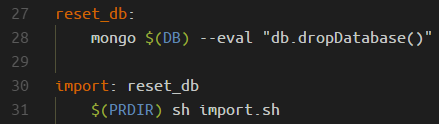
\includegraphics[scale=0.7]{img/import.png}
	\end{center}

	Le variabili \texttt{\$(DB)} e \texttt{\$(PRDIR)} sono specifiche dell'ambiente predisposto\footnote{per un esempio pratico, si consulti l'intero \texttt{makefile} riportato in \ref{appendix:makefile}.}. Essa si può lanciare con il seguente semplice comando di \texttt{shell}:

	\begin{lstlisting}[language=bash,caption={importazione dei dati in MongoDB}]
		make import
	\end{lstlisting}

	\vspace{0.3cm}

	La vera e propria invocazione del comando necessario all'import dei file nel database --- \texttt{mongoimport}, del pacchetto \texttt{mongodb-tools} --- è stata delegata in un file esterno al \texttt{makefile}, per preservare la compattezza e la brevità di quest'ultimo. Si veda comunque di seguito come è struturata la chiamata a \texttt{mongoimport} per uno degli otto file: 

	\begin{lstlisting}[language=bash,caption={dettaglio dell'importazione dei dati in MongoDB}]
		mongoimport -d exams -c rawStudentsPr1013 --type csv --file ../raw/prod_stud_10-11-12-13.csv --headerline
	\end{lstlisting}

	\vspace{0.3cm}

	Il comando, come ogni chiamata da \texttt{shell}, ha degli argomenti che ne specificano il comportamento. In questo caso, sono:

	\begin{itemize}
		\item \texttt{-d}: il database nel quale importare i dati;
		\item \texttt{-c}: la collection nella quale inserire i dati;
		\item \texttt{-type}: il tipo del file da leggere;
		\item \texttt{-file}: il riferimento al file;
		\item \texttt{--headerline}: indica che gli attributi delle istanze sono specificati nella prima riga del file.
	\end{itemize}

	A questo punto, nel database \texttt{exams} di MongoDB ci sono otto \textit{collections}, contenenti i \textit{documenti} che rappresentano le istanze dei dati a disposizione.

\section{Aggregazione per Anno Accademico}

	Avendo predisposto tutto, si può procedere con la prima lavorazione da fare. \\
	
	Si comincia intanto con l'ottenere dei data set \textit{minimali}, uno per le valutazioni dei corsi, l'altro per la produttività degli studenti, condensando in essi le informazioni principali contenute in quello delle prestazioni degli studenti in pochi parametri relativi ad un certo anno accademico. \\

	\subsection{Produttività degli Studenti}

		L'obiettivo è sintetizzare le informazioni sulla produttività degli studenti nei seguenti attributi:

		\begin{itemize}
			\item coorte di immatricolazione;
			\item numero di studenti totali;
			\item percentuale di studenti laureati;
			\item valutazione media ottenuta al test di ingresso;
			\item voto medio ottenuto agli esami;
			\item ritardo medio con cui è stato dato un esame.
		\end{itemize}

		Considerando il tipo dei dati a disposizione, occorrerà innanzitutto aggregare le istanze dei vari studenti in modo opportuno. Questo viene fatto utilizzando un modulo Python programmato \textit{ad hoc}, del quale si riporta di seguito una significativa porzione a titolo di esempio: \\

		\lstinputlisting[language=python,firstline=26,lastline=77, caption={mymodules/aggregs.py}]{../prepr/mymodules/aggregs.py}

		\vspace{0.3cm}

		L'oggetto definito nella porzione di codice appena mostrata viene impiegato per realizzare una prima aggregazione per corsi dei risultati dei singoli studenti. Si può usare questo risultato intermedio per ricavare le informazioni prefissate come necessarie, usando un altro apposito script Python: \\

		\lstinputlisting[language=python, caption={dataset\_stud\_gen.py}]{../prepr/dataset_stud_gen.py}

		\vspace{0.3cm}

		Questo codice produce una \textit{collection} che contiene esattamente il data set che ci si è prefissati di ottenere, calcolando un ritardo 	approssimativo medio (in semestri), la percentuale di studenti che hanno finito il corso di laurea nell'arco temporale a disposizione e le varie medie 	degli altri attributi.\\

		\begin{tabular}{llllll}
		\hline
		Coorte & N. & Laureati {[}\%{]} & Test Ingresso & Voto & Ritardo \\ \hline
		2010 & 30 & 6.67 & 15.4 & 25.5 & 0.81 \\
		2011 & 39 & 10.26 & 13.26 & 24.81 & 1.07 \\
		2012 & 58 & 25.86 & 14.05 & 24.79 & 1.01 \\
		2013 & 80 & 11.25 & 14.39 & 24.98 & 0.77 \\ \hline
		\end{tabular}

		\vspace{0.3cm}

		Il lancio di tutte queste operazioni è descritto nella ricetta \texttt{stud\_gen} del \texttt{makefile}.

	\subsection{Valutazione degli Insegnamenti}

		Analogamente a quanto fatto nella sezione immediatamente precedente, per questa famiglia di dati si vuole ottenere una aggregazione che riassuma i seguenti attributi:

		\begin{itemize}
			\item anno accademico
			\item numero di valutazioni registrate
			\item valutazione complessiva media dei corsi
			\item deviazione standard delle valutazioni
			\item percentuale delle valutazioni sufficienti
		\end{itemize}

		In questo caso è tutto più semplice, in quanto i dati relativi alla valutazione dei corsi sono già in forma aggregata: si tratta quindi solo di comprimerli ulteriormente, facendoli rientrare nello schema che ci si è prefissati. A tale proposito, si utilizzerà ancora il modulo \texttt{aggregs.py}, impiegandone stavolta un oggetto diverso:

		\lstinputlisting[language=python,firstline=172,lastline=259, caption={mymodules/aggregs.py}]{../prepr/mymodules/aggregs.py}

		\vspace{0.3cm}

		Dopo aver usato opportunamente l'oggetto \texttt{ParAggregator}, che mantiene nella \textit{chiave primaria} i corsi, occorre aggregare ancora i dati, rendendo l'Anno Accademico l'unico parametro in grado di discriminare una tupla dall'altra.

		\lstinputlisting[language=python, caption={dataset\_eval\_gen.py}]{../prepr/dataset_eval_gen.py}

		\vspace{0.3cm}

		Il lancio combinato di queste porzioni di codice, specificato con la ricetta \texttt{teval\_gen} del \texttt{makefile}, produce un data set di questo tipo:\\

		\begin{tabular}{lllll}
		\hline
		A. A. & Val. Media & Std. Dev. Val. & Val. Sufficienti {[}\%{]} & N. \\ \hline
		2010-2011 & 7.54 & 1.74 & 82.14 & 17 \\
		2011-2012 & 7.93 & 1.61 & 90.68 & 26 \\
		2012-2013 & 7.98 & 1.7 & 90.55 & 30 \\
		... & ... & ... & ... & .. \\ \hline
		\end{tabular}

		\vspace{0.3cm}

\section{Join dei due insiemi di dati}

	Il \textit{join} delle due famiglie di dati è l'operazione più delicata fra quelle di tutto il \textit{preprocessing}. Occorre definire bene gli attributi sui quali definire la relazione, e prestare in generale attenzione ai vari errori che, se commessi, comprometterebbero totalmente il significato del risultato. \\

	\subsection{Join con valutazioni estese e attributi continui}

		Per prima cosa, si è realizzata una \textit{join} fra i due data set aggregando i dati degli studenti \textbf{per esame}, e i dati delle valutazioni dei corsi \textbf{per paragrafo}. Osservando l'albero delle dipendenze specificato nel \texttt{makefile} riportato in \ref{appendix:makefile}, si può notare che sono state prima realizzate le aggregazioni dei singoli data set e, solo successivamente, performata l'operazione di \textit{join} fra di essi. \\

		L'aggregazione dei dati degli studenti avviene in modo del tutto analogo a quanto fatto nella sezione precedente con l'oggetto \texttt{StudAggregator} del modulo Python \texttt{aggregs.py}. \\

		Per quanto riguarda l'aggregazione dei dati delle valutazioni dei corsi, sono state effettuati vari passaggi per arrivare ad aggregare ... descritti in \ref{appendix:teval}. \\

		Predisposti opportunamente i due insiemi di dati in due \textit{collection}, la fase di merge è stata portata avanti grazie all'ausilio di un altro modulo Python scritto \textit{ad hoc}: si tratta dell'oggetto \texttt{Merger}, contenuto nel file \texttt{merge.py}, il cui codice è riportato qui sotto:

		\lstinputlisting[language=python, caption={mymodules/merge.py}]{../prepr/mymodules/merge.py}

		Tale oggetto viene utilizzato nello script \texttt{dataset\_merge.py}. Il \textit{join} avviene, chiaramente, sugli attributi \textbf{Anno Accademico} e \textbf{Corso d'Esame}, trasferendo gli attributi specifici di una collezione direttamente nell'altra in questo modo:

		\lstinputlisting[language=python, caption={dataset\_merge.py}]{../prepr/dataset_merge.py}

		A questo punto, la collezione risultante da queste operazioni ha le caratteristiche cercate. Tuttavia, presenta delle "sbavature" che è conveniente rimuovere prima di impiegarla efficacemente nel \textit{data mining}. Per eliminarle, ci si avvale di un ulteriore modulo Python realizzato per l'occasione, \texttt{cleanings.py}, il cui codice viene omesso in questa sezione per ragioni di brevità\footnote{Tale codice è comunque riportato in \ref{appendix:clean}}. \\

		Tutte queste operazioni sono invocate tramite le seguenti ricette, definite nel \texttt{makefile}:
		
		\begin{center}
			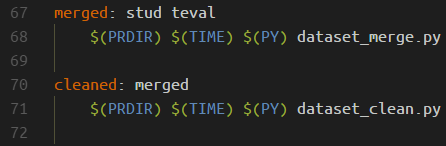
\includegraphics[scale=0.7]{img/join.png}
		\end{center}

		Concluso quanto appena descritto, si è creato un primo data set utilizzabile. Esso presenta i seguenti attributi, tutti di tipo	\textit{continuo} --- tranne ovviamente le \textit{chiavi primarie} e le istanze considerate per la produttività degli studenti:

		\begin{itemize}
			\item Anno Accademico
			\item Hash Docente/i
			\item Insegnamento
			\item \textbf{Produttività Studenti}:
				\subitem N [istanze]
				\subitem Ritardo >=1sem [percent]
				\subitem Ritardo [semestre, media]
				\subitem Voto >= 24 [perc]
				\subitem Voto [media]
				\subitem Voto [std dev]
			\item \textbf{Valutazione degli Aspetti Specifici del Corsi di Studi}:
				\subitem N [istanze]
				\subitem Std Dev [media pesata]
				\subitem Val >= 6 [percent]
				\subitem Val [media pesata]
			\item \textbf{Valutazione dell'adeguatezza delle Aule e delle Attrezzature}:
				\subitem \textit{attributi identici alla valutazione precedente}
			\item \textbf{Valutazione sul Docente}:
				\subitem \textit{attributi identici alla valutazione precedente}
			\item \textbf{Valutazione sulla Disponibilità di Informazioni Aggiuntive}:
				\subitem \textit{attributi identici alla valutazione precedente}
			\item \textbf{Valutazione dell'Organizzazione del Corso di Studi}:
				\subitem \textit{attributi identici alla valutazione precedente}
			\item \textbf{Valutazione dell'Organizzazione della Didattica}:
				\subitem \textit{attributi identici alla valutazione precedente}
			\item \textbf{Soddisfazione degli Studenti riguardo al Corso di Studi}:
				\subitem \textit{attributi identici alla valutazione precedente}
		\end{itemize}

		Come si può notare agilmente, il data set presenta un gran numero di attributi, molti fin troppo specifici per poterne estrarre un qualche tipo di informazione generale. Pertanto, è stato deciso aggregare ulteriormente fra loro gli attributi relativi alle valutazioni dei corsi, per sfoltire significativamente la quantità di campi presenti.
		
	\subsection{Join con valutazioni aggregate e attributi continui}
	
	\subsection{Attributi discreti}

\section{Sequenze ordinate di esami superati}

\section{Estrazione dei data set preprocessati}

	\begin{center}
		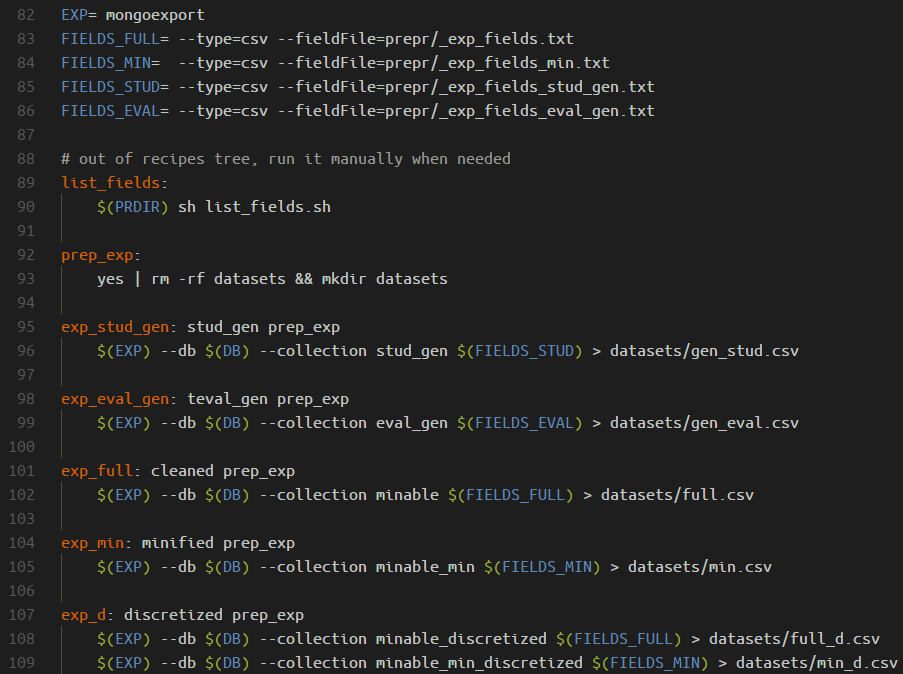
\includegraphics[scale=0.7]{img/export.png}
	\end{center}

	\lstinputlisting[language=bash,caption={script di shell per ottenere una lista degli attributi dei documenti in una collezione}, numbers=left, stepnumber=1]{../prepr/list_fields.sh}

	\lstdefinelanguage{JavaScript}{
  		keywords={break, case, catch, continue, debugger, default, delete, do, else, finally, for, function, if, in, instanceof, new, return, switch, this, throw, try, typeof, var, void, while, with},
 		morecomment=[l]{//},
  		morecomment=[s]{/*}{*/},
  		morestring=[b]',
  		morestring=[b]",
  		sensitive=true
	}

	\lstinputlisting[language=JavaScript,caption={script della shell di MongoDB per ottenere la lista degli attributi dei documenti in una collezione}, numbers=left, stepnumber=1]{../prepr/list_attr.mongosh}
